\documentclass[10pt]{article}

\usepackage{times}
%\usepackage{mathptmx}
\usepackage{amsmath}
%\usepackage{mathtools}
\usepackage{graphicx}


\title{Time-discrete Stochastic Signals\\
Lab report in TSDT14}

\author{Erik H Kjellman eriha181, 881227-1958 \and
Klara Wingstedt klawi021, 890823-2724 }

\date{\today}

\begin{document}

\maketitle

\newpage

\section{Introduction}

\subsection{Study 1 --- Modeling signals}
The objective of the first study is to model a stochastic signal
and filter it through two separate digital filters, one of which will 
be close to an ideal low-pass filter, and the other a simple low-degree 
low-pass filter that is easily analysed by hand. 

The auto-correlation function (ACF) and power spectral density function (PSD) will also be calculated, and compared to the theoretical results. 

\subsection{Study 2 --- Non-LTI-systems}
The goal in this part is similar to the first study, but the stochastic signal will now be filtered through three different kinds of non-linear filters.

\subsection{Study 3 --- Special Operations}
The task in this study is to investigate what happens to the power spectral density (PSD) in two different special cases. 

\section{Study 1 --- Modeling signals}
White Gaussian noise, referred to as WGN from hereon out, was generated in Matlab and filtered through two separate filters given by these equations.

\begin{align*}
H_{\text{simple}} = \frac{1}{1 + i\frac{f}{f_c}}
\end{align*}

\begin{align*}
H_{\text{ideal}} = rect(\frac{f}{f_c})
\end{align*}

Where $H_\text{ideal}$ is approximated by a high order Butterworth filter.

\subsection{ACF and PSD}
\subsubsection{Theoretical functions}
The PSD function of WGN is a constant $R_x$ which has been chosen as $R_x = 1$ for simplicity. The PSD of the filtered signal is then given by

\begin{align*}
R_y = R_x|H(f)|^2
\end{align*}

and the ACF is given by the inverse Fourier transform of $R_y$

\begin{align*}
r_y[n] = \mathcal{F}^{-1}{R_y}[n]
\end{align*}

\subsubsection{Estimated functions}
The ACF was calculated using the Bartlett's estimate,
\begin{align*}
\hat{r}_y[k] &=  \frac{1}{N}\sum_{n=0}^{N-|k|-1}r_x[n+|k|]r_x[n]
\end{align*}

and the PSD was calculated from the estimated ACF via the Fourier transform.
To get nicer plots, averaging and smoothing were applied as well.

\begin{figure}[!hp]

    \begin{center}
      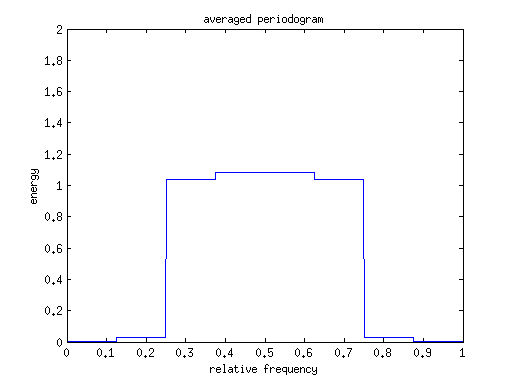
\includegraphics[width=1\textwidth]{ideal_periodogram_average}
    \caption{PSD of $y_\text{ideal}$, with averaging. \label{fig:TheoACFsimple}}
    \end{center}

\end{figure}

\begin{figure}[!hp]

    \begin{center}
      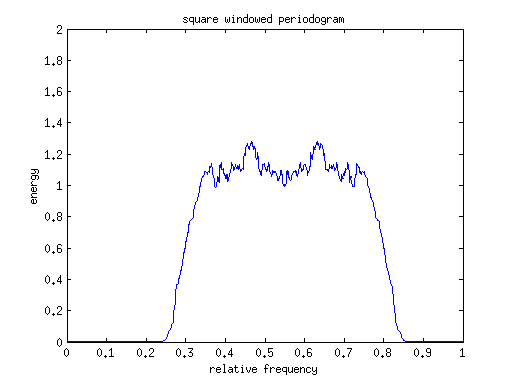
\includegraphics[width=1\textwidth]{ideal_periodogram_square}
    \caption{PSD of $y_\text{ideal}$, with smoothing with a square window. \label{fig:TheoACFsimple}}
    \end{center}

\end{figure}

\begin{figure}[!hp]

    \begin{center}
      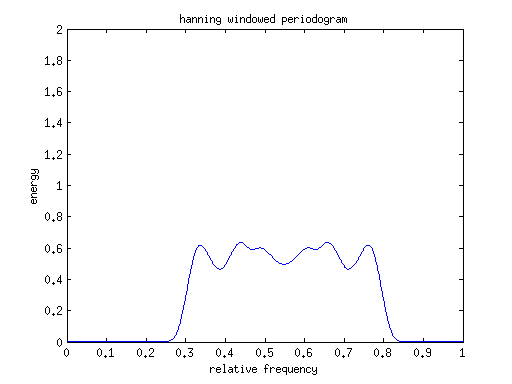
\includegraphics[width=1\textwidth]{ideal_periodogram_hanning}
    \caption{PSD of $y_\text{ideal}$, with smoothing with a hanning window. \label{fig:TheoACFsimple}}
    \end{center}

\end{figure}


\begin{figure}[!hp]
    \begin{center}
      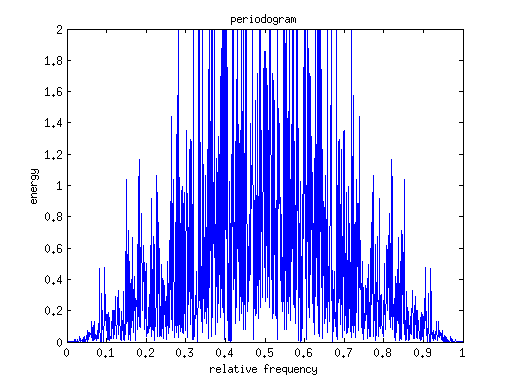
\includegraphics[width=1\textwidth]{simple_periodogram}
    \caption{PSD of $y_\text{simple}$. \label{fig:TheoACFsimple}}
    \end{center}
\end{figure}

\begin{figure}[!hp]
    \begin{center}
      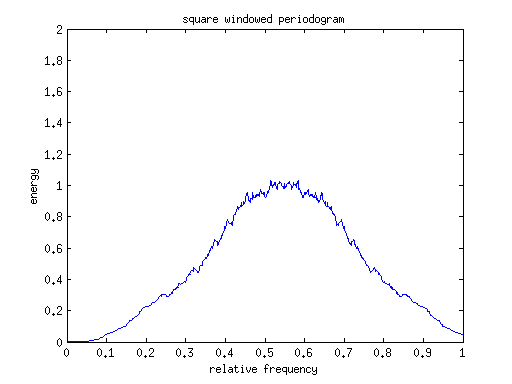
\includegraphics[width=1\textwidth]{simple_periodogram_square}
    \caption{PSD of $y_\text{simple}$, smoothed with a square window. \label{fig:TheoACFsimple}}
    \end{center}
\end{figure}

\begin{figure}[!hp]
    \begin{center}
      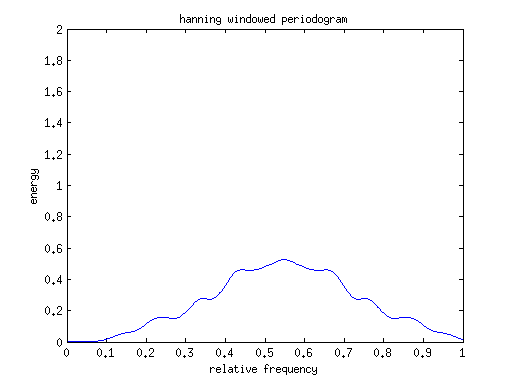
\includegraphics[width=1\textwidth]{simple_periodogram_hanning}
    \caption{PSD of $y_\text{simple}$, smoothed with a hanning window. \label{fig:TheoACFsimple}}
    \end{center}
\end{figure}


\subsection{Comparisons and conclusions}
The ACF is in no dire need of improvement, since the dirac spike is clearly visible, though there is a difference in higher k values compared to the theoretical function, where the theoretical function is zero.

The PSD on the other hand has much to gain from further improvements, which can clearly be seen in the plots. The theoretical PSD is just a rectangle function, which the averaged PSD is very close to.


\section{Study 2 --- Non-LTI-systems}
WGN was again generated and filtered through a high-degree filter as in Study 1, but now this filtered noise shall be used as an input to three different systems, a squarer, a half-wave rectifier and an AM-SC modulator:

\begin{align*}
  Y_\text{sq}[n] =X^2[n]
\end{align*}

\begin{align*}
  Y_\text{HW}[n] =
\begin{cases}
   X[n],& n: X[n]>0,\\
    0,    & n: X[n] \leq 0
\end{cases}
\end{align*}

\begin{align*}
  Y_\text{AM-SC}[n] =X[n]cos(\Omega_{0}n)
\end{align*}

Some properties of LTI systems don't hold for non-LTI systems, among others that Gaussian input doesn't always imply Gaussian output, and that the filter can introduce new frequencies that weren't present in the input.

As can be seen in the PSD plots below, new frequencies have been introduced in each of the filters, less so in the half-wave case, but it's still clearly visible.


\begin{figure}[!hp]
    \begin{center}
      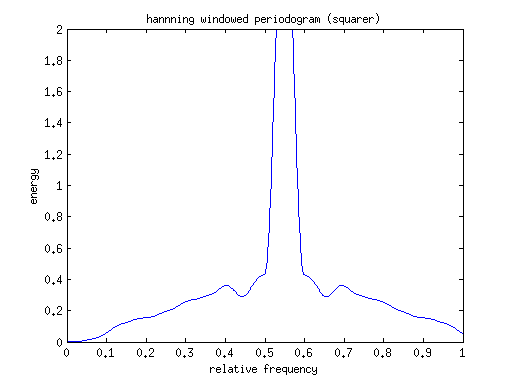
\includegraphics[width=1\textwidth]{ideal_periodogram_hanning_squarer}
    \caption{PSD of $y_\text{sq}$, smoothed with a hanning window. \label{fig:TheoACFsimple}}
    \end{center}
\end{figure}

\begin{figure}[!hp]
    \begin{center}
      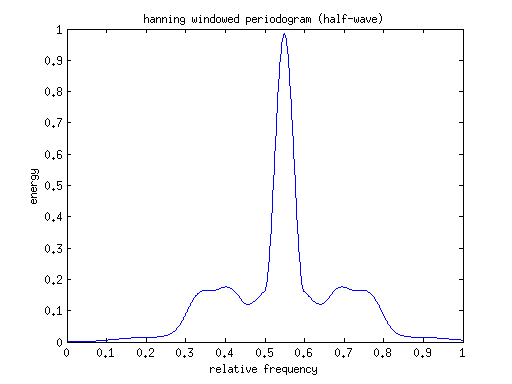
\includegraphics[width=1\textwidth]{ideal_periodogram_hanning_half-wave}
    \caption{PSD of $y_\text{HW}$, smoothed with a hanning window. \label{fig:TheoACFsimple}}
    \end{center}
\end{figure}

\begin{figure}[!hp]
    \begin{center}
      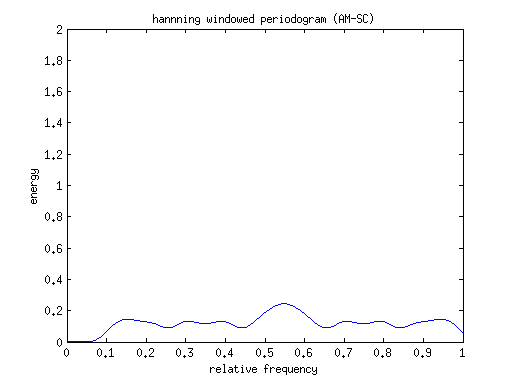
\includegraphics[width=1\textwidth]{ideal_periodogram_hanning_AM-SC}
    \caption{PSD of $y_\text{AM-SC}$, smoothed with a hanning window. \label{fig:TheoACFsimple}}
    \end{center}
\end{figure}

\newpage
As stated previously, non-LTI systems doesn't necessarily adhere to the rule that Gaussian input implies Gaussian output, which LTI systems must. It is visible in the following figures of amplitude distribution that each of the filters in this study don't follow this rule.

\begin{figure}[!hp]
    \begin{center}
      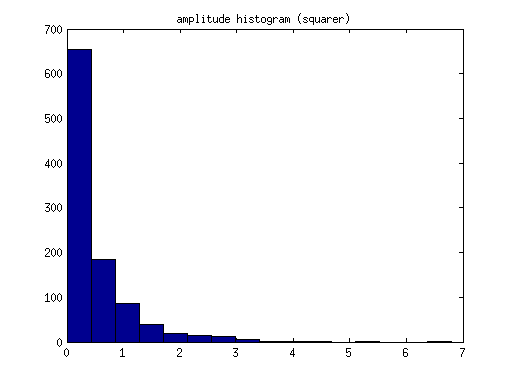
\includegraphics[width=1\textwidth]{amplitude_histogram_squarer}
    \caption{Amplitude histogram of $y_\text{sq}$. \label{fig:TheoACFsimple}}
    \end{center}
\end{figure}


\begin{figure}[!hp]
    \begin{center}
      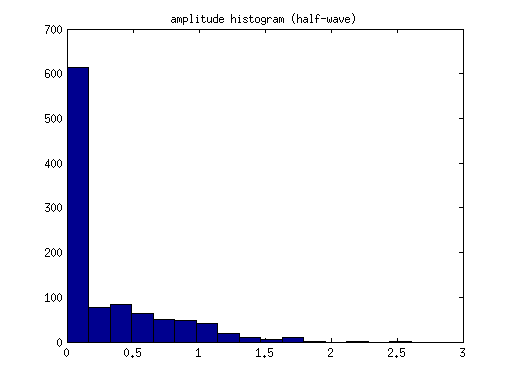
\includegraphics[width=1\textwidth]{amplitude_histogram_half-wave}
    \caption{Amplitude histogram of $y_\text{HW}$. \label{fig:TheoACFsimple}}
    \end{center}
\end{figure}

\begin{figure}[!hp]
    \begin{center}
      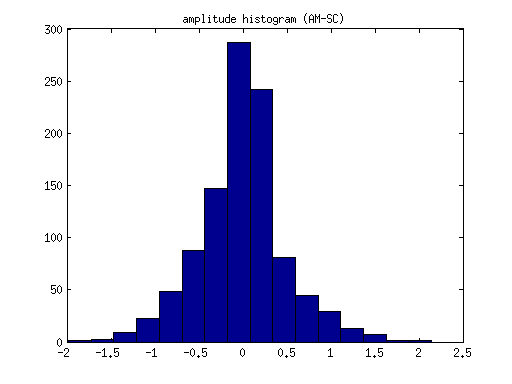
\includegraphics[width=1\textwidth]{amplitude_histogram_AM-SC}
    \caption{Amplitude histogram of $y_\text{AM-SC}$. \label{fig:TheoACFsimple}}
    \end{center}
\end{figure}

\newpage
\section{Study 3 --- Special Operations}
In this study, the output from the approximated ideal filter will be used as input to two different systems. The first is described by

\begin{align*}
Y[n] = X[n](-1)^2
\end{align*}

and the second is a decimation, which means that every second sample is replaced by a zero. The theoretical ACF's and PSD's are arrived at the equations given below.



\begin{align*}
r_{dec}[k] & =\frac{1}{4}r_X[k](1+(-1)^k)
\end{align*}

\begin{align*}
R_{dec}[\theta] & = \mathcal{F}\{r_{dec}[k]\} \nonumber \\
& = \frac{1}{4}(R_X[\theta]+R_X[\theta-0.5]) \nonumber \\
& = \frac{1}{4}(rect(\frac{\theta-0.5}{2\theta_c}) + rect(\frac{\theta}{2\theta_c}))
\end{align*}

\begin{align*}
r_{alt}[k] & = E\{X[n+k](-1)^{n+k}X[n](-1)^n\} \\
& =r_X[k](-1)^k
\end{align*}

\begin{align*}
R_{alt}[\theta] & = \mathcal{F}\{r_{alt}[k]\} \nonumber \\
& = R_X[\theta-0.5] = rect(\frac{\theta-0.5}{2\theta_c})
\end{align*}



\begin{figure}[!hp]
    \begin{center}
      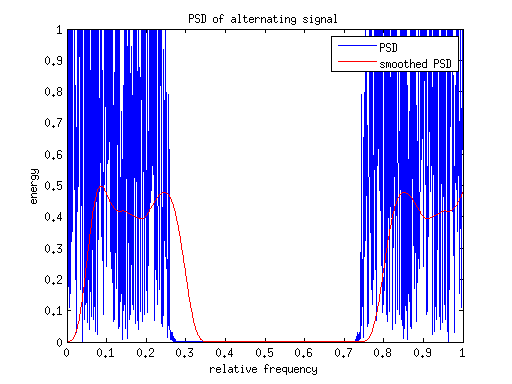
\includegraphics[width=1\textwidth]{ideal_periodogram_hanning_alternating}
    \caption{PSD of alternating function, both smoothed with a hanning window and untouched. $y_\text{sq}$. \label{fig:TheoACFsimple}}
    \end{center}
\end{figure}

\begin{figure}[!hp]
    \begin{center}
      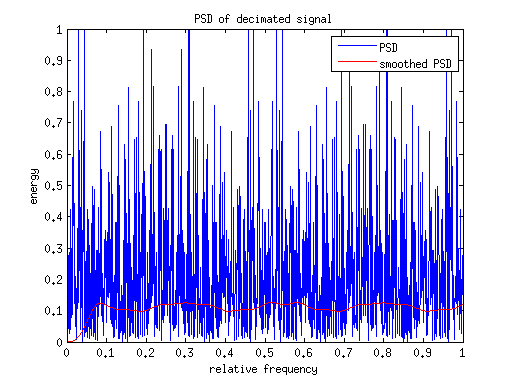
\includegraphics[width=1\textwidth]{ideal_periodogram_hanning_decimated}
    \caption{PSD of decimated function, both smoothed with a hanning window and untouched. $y_\text{sq}$. \label{fig:TheoACFsimple}}
    \end{center}
\end{figure}

The theoretical and practical results are corresponding well, which is of course more easily visible in the smoothed versions of the PSD's.


\end{document}
